\documentclass[11pt]{article}

\usepackage{graphicx}
\usepackage[T1]{fontenc}
\usepackage{amssymb}
\usepackage{amsthm}
\usepackage{enumerate}
\usepackage{amsmath}
\usepackage{mathrsfs}
\usepackage{braket}
\usepackage{dsfont}
\usepackage{braket}
\usepackage{siunitx}
\sisetup{load-configurations = abbreviations}
\usepackage{hyperref}

\usepackage{geometry}
\geometry{%
  letterpaper,
  lmargin=2cm,
  rmargin=2cm,
  tmargin=2cm,
  bmargin=2cm,
  footskip=12pt,
  headheight=12pt}

\date{}
\title{\vspace{-3cm} PHYS 334 - Notes \\ \large Anton Borissov \vspace{-1cm} }
\author{}

\makeatletter
\def\imod#1{\allowbreak\mkern10mu({\operator@font mod}\,\,#1)}
\makeatother

\newcommand{\Z}{\mathbb{Z}}
\renewcommand{\H}{\hat{H}}
\newcommand{\comp}{\circ}
\newcommand{\lcm}{\text{lcm}}
\newcommand{\N}{\mathbb{N}}
\newcommand{\Q}{\mathbb{Q}}
\newcommand{\R}{\mathbb{R}}
\newcommand{\C}{\mathbb{C}}
\newcommand{\D}{\mathbb{D}}
\newcommand{\X}{\mathscr{X}}
\newcommand{\ZZ}{\mathbb{Z}[\sqrt{2}]}
\newcommand{\QQ}{\mathbb{Q}[\sqrt{2}]}
\newcommand{\tat}{\text}
\newcommand{\normal}{\trianglelefteq}
\newcommand{\ti}{\to\infty}
\newcommand{\mc}{\mathcal}
\newcommand{\cnj}{\overline}
\newcommand{\pres}[1]{\langle #1 \rangle}

\newcommand{\eps}{\epsilon}
\newcommand{\guillemot}[1]{\guillemotleft{#1}\guillemotright}
\newcommand{\vnabla}{\vec\nabla}

\renewcommand{\vec}[1]{\mathbf{#1}}
\newcommand{\hv}[1]{\hat{\mathbf{#1}}}
\newcommand{\dv}[1]{\dot{\mathbf{#1}}}
\newcommand{\ddv}[1]{\ddot{\mathbf{#1}}}

\newcommand{\FR}[2]{\frac{#1}{#2}}
\newcommand{\PP}[2]{\frac{\partial #1}{\partial #2}}
\newcommand{\LL}{\left}
\newcommand{\RR}{\right}

\newcommand{\iden}{\mathds{1}}

\theoremstyle{plain}
\newtheorem{thm}{Theorem}[section] 
\newtheorem{lem}[thm]{Lemma}
\newtheorem{post}[thm]{Postulate}

\theoremstyle{definition}
\newtheorem{defn}{Definition}
\newtheorem{conj}{Conjecture}
\newtheorem{ex}{Example}

\theoremstyle{remark}
\newtheorem*{remark}{Remark}
\newtheorem*{note}{Note}
\newtheorem{case}{Case}

\DeclareMathOperator{\spec}{Spec}
\DeclareMathOperator{\Sym}{Sym}
\DeclareMathOperator{\Span}{span}
\DeclareMathOperator{\im}{im}
\DeclareMathOperator{\nullity}{nullity}
\DeclareMathOperator{\rank}{rank}
\DeclareMathOperator{\id}{id}
\DeclareMathOperator{\real}{Re}
\DeclareMathOperator{\Aut}{Aut}
\DeclareMathOperator{\Tr}{Tr}
\let\div\relax
\DeclareMathOperator{\div}{div}

\def\bE{\begin{enumerate}}
\def\eE{\end{enumerate}}
\def\ii{\item}

\DeclareSIUnit\Ry{Ry}

\begin{document}
\subsection{Preliminaries}
\begin{align*}
\hbar   &= \SI{1.05e-34}{\joule\s}\\
\hbar c &= \SI{297.3}{\eV.\nm}\\
m_e     &= \SI{0.511}{\MeV.\nm}\\
\FR{e^2}{4\pi\eps_0} &= \SI{1.44}{\eV\nm}\\
\alpha = \FR{e^2/4\pi\eps_0}{\hbar c} &\sim \FR{1}{137}\\
hc &= \SI{1240}{\eV\nm}\\
\SI{1}{\amu} &= 930\si{MeV/c^2}\\
a_0 &= \SI{0.05}{\nm} = \SI{0.5}{\angstrom}\\
\SI{1}{\Ry} &= \SI{-13.6}{\eV}\\
k_B T &= \SI{0.025}{\eV} (T \sim 290)
\end{align*}

\subsubsection{Back of the envelope Calculation - Bohr radius and Rydberg energy}
Find $a_0$ and $\SI{1}{\Ry}$: $dpdx \sim \hbar \implies p \sim dp \sim
\FR{\hbar}{a_0}$. Now minimizing the energy: $E = \FR{p^2}{2m_e}-
\FR{e^2/4\pi\eps_0}{a_0} \sim \FR{\hbar^2}{2ma_0^2}-\FR{e^2/4\pi\eps_0}{a_0}$
gives $E_{min}$ at $a_0 = \FR{\hbar^2}{me^2/4\pi\eps_0}
= \FR{\hbar^2c^2}{mc^2 \cdot e^2/4\pi\eps_0}
= \FR{300^2}{0.511 \cdot 1.44}
= \SI{0.5}{\angstrom}$.

\subsection{Introduction}
Any square integrable function $\Psi(\vec r,t)$ describes a state of
the system. It is called a probability density because the probability
of finding a particle in a volume $\vec r \pm d^3 r$ at a fixed time $t$
is \[ d^3 r |\Psi(\vec r,t)|^2 \]

Moreover any superposition, that is a linear combination, also
represents a state. Time evolution of a state is given by the
Time-dependent Schrodinger equation. This equation is the
\guillemot{simplest} PDE that satisfies:
\bE
\ii Einstein ($E=\hbar \omega$) and deBroglie ($p=\hbar/\omega$)
\ii $E = \FR{p^2}{2m} + V(\vec r,t)$.
\ii Linear in $\Psi$.
\eE
This gives $i\hbar \PP{\Psi}{t} = \hat H\Psi$.

\subsubsection{Continuity Equation}
Derivation gives: 
$\vec J = \FR{\hbar i}{2m} (\Psi\nabla\Psi^* - \Psi^*\nabla\Psi)$,
\[\FR{P(\vec r,t)}{t} + \div\vec J = 0\]

\begin{align*}
\FR{d}{dt}\int d^3 r P(\vec r,t) &= - \oint ds \vec J \cdot \hv n\\
\vec J &= \FR{1}{2m}\LL[ \Psi^* \FR{\hbar}{i} \vnabla \Psi
+(\Psi^*\FR{\hbar}{i} \vnabla \Psi)^*\RR]\\
&= \FR{1}{m}\Re\LL[\Psi^*\FR{\hbar}{i} \vnabla \Psi\RR]
\end{align*}

In the case of a plane wave, $\Psi = 
A e^{i \LL[ \FR{\vec p\vec r - E_p t}{\hbar}\RR]}$ gives
$\vec J = |A|^2 \FR{\vec p}{m}$ (cf. fluid mechanics).

To show that $\hat H$ is hermitian:
\begin{align*}
0 &= \FR{d}{dt} \int d^3 r P(\vec r,t)
&= \FR{d}{dt} \int d^3 r -\div J\\
&= \cdots\\
&\int d^3 r \Psi^*(H-H^*)\Psi
\end{align*}
Since this works for all $\Psi$, $H-H^* = 0$ thus $H^*$ is
Hermitian. Note that in this class we \emph{define}
an operator $A$ to be Hermitian if it satisfies:
\[ \int d^3 r \Psi^* \hat A \Psi =
 = \int d^3 r \Psi (\hat A \Psi)^* \]

\subsection{Time independence}
Assume that $V(\vec r,t) = V(\vec r)$ and $\Psi = \psi(\vec r)\chi(t)$.
\begin{align*}
i\hbar \PP{\Psi}{t} &= H\Psi\\
i\hbar \psi(\vec r)\FR{d\chi}{dt} &= [H\psi]\chi\\
i\hbar \FR{d\chi}{\chi} &= \FR{1}{\psi}[H\psi]
\end{align*}
The LHS is a function of time and the RHS is a function of $\vec r$.
Therefore both are constant. Let $E$ be this constant:
\begin{align*}
i\hbar \FR{d\chi}{\chi} &= E & H\Psi = E\Psi\\
\chi(t) &= e^{-i (Et/\hbar)}&\\
    \therefore \Psi(\vec r,t) &= \psi(\vec r)e^{-i(Et/\hbar)}
\end{align*}

\subsubsection{Free Particle}
In the case of a free particle, $V \equiv 0$ and so by solving we will
get in one dimension: $\Psi(x,t) = e^{i(px-\FR{p^2}{2m}t)/\hbar}$.
Strange things happen:
\bE
\ii Speed of a wave is given by the solution to the phase being constant.
(Imagine sitting on top of a peak. In this frame, the phase at any given point
does not move.) Therefore the speed of this particle is given by:
\[ px -\FR{p^2}{2m} \equiv \text{const} \implies \FR{dx}{dt} = \FR{p}{2m} \]
which is half of the \guillemot{expected} velocity.
\ii Normalization of $\Psi$ is not possible.

One solution to this problem is to put the particle in a large box:
$-L \le x \le L$, impose suitable boundary conditions and let 
$L \to \infty$ at the end of the calculation.\footnote{This will appear in
solid state physics and condensed matter physics.}

A more physical approach would be to treat $\Psi(x,t) = A e^{i(px-\FR{p^2}{2m})/\hbar}$
as a tool so that we can decompose a state $\Psi$ using a momentum eigenbasis:
\[\Psi(x,t) = \int dp\, A_p e^{ipx/\hbar} e^{-iE_p t/\hbar}\]
For convenience we can set $A_p = \FR{1}{\sqrt{2\pi\hbar}}\phi(p)$ to
\[\Psi(x,t) = \FR{1}{\sqrt{2\pi\hbar}}\int dp \phi(p) e^{-i(px+E_pt)/\hbar}\]
\eE

\subsubsection{Fourier Playground}

Now, that we have two different descriptions of $\Psi(x,t)$:
$\Psi(x,t) = \FR{1}{\sqrt{2\pi\hbar}}\int dp \phi(p) e^{-i(px+E_pt)/\hbar}
           = \psi(x)e^{-i(Et/\hbar)}$,
we may use the fourier transform to swap between these two representations.

\begin{thm}\label{FIT}
\footnote{In classical wave mechanics $k$ denotes the wave number.
    Need an appendix on the Fourier transform. Consult wikipedia at:
    \url{http://en.wikipedia.org/wiki/Fourier_transform}
and \url{http://en.wikipedia.org/wiki/Uncertainty_principle}}
If $f\in L^2$ (square integrable) and both $f$ and $f'$ are piecewise continuous
then \[ f(x) = \FR{1}{\sqrt{2\pi}}\int F(k) e^{ikx} dk \] where
\[F(k) = \FR{1}{\sqrt{2\pi}}\int f(x) e^{-ikx}dx.\]
\end{thm}

By setting $k = \FR{p}{\hbar}$ we get $f(x) \to \psi(x)$ and 
$F(k) \to \sqrt{\hbar}\phi(p)$.

Suppose we put a particle into a box, $-a < x < a$ with
$\Psi(x,0) = \psi(x) = \begin{cases} \FR{1}{\sqrt{2a}} &-a<x<a\\ 0 & x\not\in(-a,a)
\end{cases}$. Then applying the FIT(\ref{FIT}) we get:
\[\phi(p) = \FR{1}{\sqrt{2a}}\int \FR{e^{-ipx}}{\sqrt{2a}}
          = \FR{1}{\sqrt{\pi\hbar}} \FR{\sin(pa/\hbar)}{p/\hbar}\]
\begin{center}
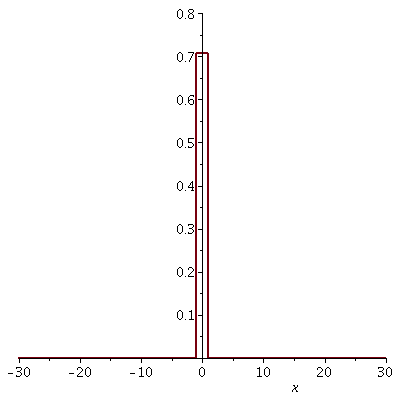
\includegraphics[scale=0.25]{posn_repn}
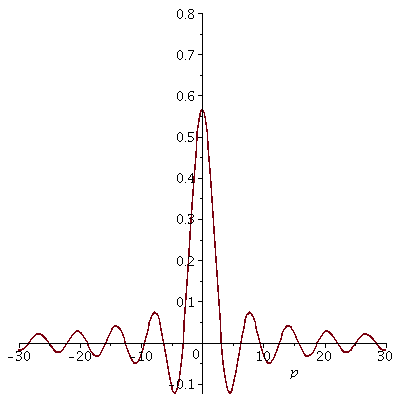
\includegraphics[scale=0.25]{mnt_repn}\end{center}

\begin{note}
This seemingly extreme behaviour above is due to the uncertainty principle.
See wiki and appendix for more details. Someone mentioned in class that the
different peaks of the position representation correspond to different energy
levels; investigate.
\end{note}

Next, we wish to model a particle with a momentum of $p_0$.
Therefore $e^{ip_0 x/\hbar}$ has the largest contribution to $\Psi(x,t)$.
Doing a first order expandsion of $E_p$:
\[ E_p = E_0 + \LL(\FR{dE}{dp}\RR)_{p_0}(p-p_0) \equiv
E_0 + E_0'(p-p_0)\]
Therefore
\begin{align*}
\Psi(x,t) &\sim \FR{1}{\sqrt{2\pi\hbar}} \int dp
\phi(p) e^{i(px-E_0t)/\hbar} e^{iE_0'(p-p_0)t/\hbar}\\
          &= e^{-i(E_0-E_0'p_0)t/\hbar}
             \int \FR{dp}{\sqrt{2\pi\hbar}} \phi(p) e^{ip(x-E_0't)/\hbar}\\
          &= e^{-i(E_0-E_0'p_0)t/\hbar} \psi(x-E_0't)
\end{align*}
Therefore the wave packet seems to be moving with group velocity $v_g = E_0'$.

A first order approximation is good if and only if the second order error is 
small: $\Delta E_2 = \FR{1}{2}\LL(\FR{d^2 E}{dp^2}\RR)_{p_0}(p-p_0)^2
= \FR{(\Delta p)^2}{2m}$. It turns out\footnote{Why?} that $\Delta E_2$
represents the spread of the wave function and so there is negligible spread
if:
\[ \FR{\Delta E_2}{\hbar} t \ll 1 \implies
   \FR{(\Delta p)^2 t}{2m\hbar} \ll 1 \implies
   \FR{\hbar t}{2m(\Delta x)^2} \ll 1\]
Let $D$ be the dimension of the apparatus in an experiment so that:
$t \sim \FR{D}{v_g} = \FR{mD}{p_0}$ and $\FR{\hbar t}{2m(\Delta x)^2} \ll 1$
gives:
\[ \FR{\hbar D}{2(\Delta x)^2p_0} \ll 1 \implies \FR{\lambda_0 D}{4\pi(\Delta x)^2} \ll 1
    \implies \FR{\Delta x}{\lambda_0} \gg \FR{D}{4\pi\Delta x}\]
Estimate: $D\sim \SI{1}{mm}, \Delta x \sim \SI{1}{nm} \implies \FR{D}{\Delta x} \gg 1$.
Now magic\footnote{justify, I don't think this statement logically follow as it should}:
thus the wave packet has negligible spread if $\Delta x/\lambda_0 \gg 1$. Thus,
the wave packet must contain many deBroglie wavelengths.

\subsection{Formal Theory}
Statement of the 6 postulates.
From P6, any measuremenet of a physical observable imply that the associated
operator is Hermitian:
\[ \int d^3 r \Psi^* \hat A \Psi = \braket{A} = \braket{A}^*
 = \int d^3 r \Psi (\hat A \Psi)^* \]


\end{document}
